\documentclass{beamer}
%
% Choose how your presentation looks.
%
% For more themes, color themes and font themes, see:
% http://deic.uab.es/~iblanes/beamer_gallery/index_by_theme.html
%
\mode<presentation>
{
  \usetheme{Warsaw}      % or try Darmstadt, Madrid, Warsaw, ...
  \usecolortheme{default} % or try albatross, beaver, crane, ...
  \usefonttheme{default}  % or try serif, structurebold, ...
  \setbeamertemplate{navigation symbols}{}
  \setbeamertemplate{caption}[numbered]
} 
\usepackage{animate}
\usepackage[english]{babel}
\usepackage[utf8]{inputenc}
\title[MCMC using Hamiltonian Dynamics]{Markov Chain Monte Carlo using Hamiltonian Dynamics}
\author{Joshua James MacDonald}
\institute{}
\date{\today}
\begin{document}

% ===============================================

\begin{frame}
  \titlepage
\end{frame}

% Uncomment these lines for an automatically generated outline.
%\begin{frame}{Outline}
%  \tableofcontents
%\end{frame}


% ===============================================

\section{Aims}

% ===============================================
\begin{frame}{Aims}

\begin{itemize}

\item Understand why Hamiltonian Monte Carlo works \vskip 5mm

\item Tuning the HMC Algorithm \vskip 5mm

\item Investigating Scaling with Dimension and Optimal Acceptance Rate 
\end{itemize}

\end{frame}

% ===============================================

\section{Hamiltonian Dynamics}

% ===============================================


\begin{frame}{Hamiltonian Parameter Space}
\begin{itemize}
\item A ball rolling around a potential surface \vskip 5mm
\item At any time the ball has position $x$ and momentum $p$ \vskip 5mm
\item Also has a mass $m$ \vskip 5mm
\end{itemize}
\end{frame}
% ==== 

\begin{frame}{A Simple Potential Surface}

\begin{figure}
\centering
\animategraphics[scale = 0.3, loop = true]{20}{Animations/First_Normal_Potential}{001}{101}
\end{figure}
\end{frame}


\begin{frame}{The Hamiltonian}
Potential Energy,
\begin{equation*}
U(x) = - \log \{\pi(x)\}
\end{equation*}

Kinetic Energy,
\begin{equation*}
K(p; m) = \frac{1}{2} \frac{p^2}{m}
\end{equation*}

The Hamiltonian,
\begin{equation*}
H(x, p; m) = U(x) + K(p;m)
\end{equation*}
\end{frame}

% ==== 
\begin{frame}{Hamiltonian Equations}

\begin{equation*}
\frac{dx}{dt} = \frac{p}{m}
\end{equation*}

\begin{equation*}
\frac{dp}{dt} = - \frac{dU}{dx}
\end{equation*}

Can be generalised to higher dimensions

\begin{equation*}
\frac{d\bf{x}}{dt} = M^{-1}\bf{p}
\end{equation*}

\begin{equation*}
\frac{d\bf{p}}{dt} = - \nabla U(\bf{x})
\end{equation*}

\end{frame}
% ==== 

\begin{frame}{1-dimensional Gaussian Example}
% Graph of N(0,1) Density
% Graph of log(N(0,1))
% Graphic of Ball rolling around -log(N(0,1))
\begin{figure}
\centering
\animategraphics[scale = 0.3, loop = true]{20}{Animations/Normal_Potential}{001}{101}
\end{figure}
\end{frame}

% ====

\begin{frame}{Approximating Hamiltonian Dynamics}

\begin{itemize}
\item Hamiltonian Dynamics are approximated using a numerical discretisation. 

\item Simulate over time $T$, using $L$ steps and stepsize $\varepsilon$

\item When used in MCMC, gives acceptance probability $$ \alpha(x^{*}, p^{*} ;x, p) = \min \Big{\{} 1, \exp(-(H(x^{*}, p^{*};M) - H(x,p;M)) \Big{\}} $$

\end{itemize}

\end{frame}





%\begin{frame}{Why Hamiltonian Dynamics?}
%\begin{itemize}
%\item Reversibility of Hamiltonian Dynamics ensures Detailed Balance. \vskip 5mm

%\item If Hamiltonian is conserved, we have acceptance probability of 1 \vskip 5mm

%\item Volume Preservation \vskip 5mm
%\end{itemize}
%\end{frame}

% ====

%\begin{frame}{Leapfrog Approximation (Störmer-Verlet)}

%\begin{itemize}
%\item A method of approximating Hamiltonian Dynamics \vskip 5mm

%\item Preserves the desirable properties of Hamiltonian Dynamics \vskip 5mm

%\item Approximately conserves the Hamiltonian \vskip 5mm

%\item $T$, Integration Time \vskip 5mm 

%\item $\varepsilon$, stepsize \vskip 5mm

%\item $L$, Leapfrog steps \vskip 5mm
%\end{itemize}

%\begin{equation}
%T = L \varepsilon 
%\end{equation}

%\end{frame}

% ===============================================
\section{HMC Algorithm}
% ==============================================

\begin{frame}{HMC Algorithm}
\begin{itemize}

\item We have some position $x$.

\item Draw a new momentum $ p \sim \mathcal{N}(0, M)$.

\item Approximate Hamiltonian Dynamics for time $T$ in $L$ steps, using stepsize $\varepsilon$. 

\item Proposes new position and momentum $(x^{*}, p^{*})$. 

\item Accept proposal with probability $$ \alpha(x^{*}, p^{*} ;x, p) = \min \Big{\{} 1, \exp(-(H(x^{*}, p^{*};M) - H(x,p;M)) \Big{\}} $$
\end{itemize}

\end{frame}


% ===============================================
\section{Tuning the HMC Algorithm}
% ===============================================


\begin{frame}{Choosing the Integration Time}

\begin{itemize}

\item The distance moved in a prosposal can be directly controlled by $T$ \vskip 5mm

\item This doesn't affect the acceptance probability \vskip 5mm

\item Hard to know what values of $T$ will be sensible

\end{itemize}

\end{frame}


\begin{frame}{Choosing a Stepsize}

\begin{itemize}

\item Error in the Approximation is controlled by the stepsize. \vskip 5mm

\item Approximation can become unstable if the chosen stepsize is too large \vskip 5mm
\end{itemize}

\begin{figure}
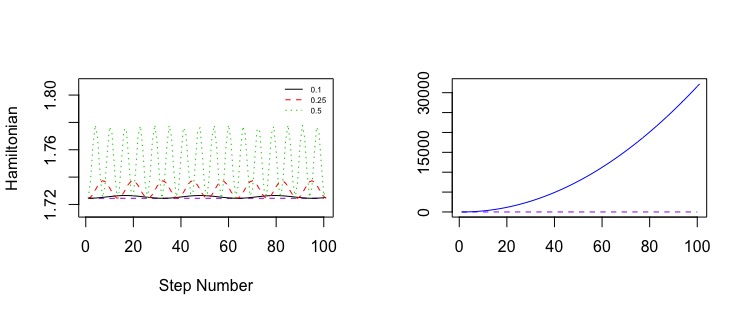
\includegraphics[scale = 0.3]{Leapfrog_Errors.jpeg}
\end{figure}

\end{frame}

% ====

\begin{frame}{Choosing the Number of Steps}

\begin{itemize}
\item  \vskip 5mm

\item Find a range of stepsizes which perform suitably \vskip 5mm
\end{itemize}

\end{frame}



% ===============================================

\section{Scaling and Optimal Acceptance Rate}

% ===============================================

\begin{frame}{Scaling and Optimal Acceptance Rate}

\begin{itemize}

\item  The Performance of MCMC in high dimensions has become important with the rise of Big Data \vskip 5mm

\item How far can we move with each proposal while keeping a reasonable acceptance rate? \vskip 5mm

\end{itemize}

\end{frame}


\begin{frame}{Scaling with Dimension}

\begin{table}
\centering
\begin{tabular}{|c||c|c|}
\hline
Algorithm & Scaling & Optimal Acceptance Rate $(d \to \infty)$ \\
\hline
RWM & $d^{-1/2}$ & $23.4\%$ (Roberts \& Rosenthal 2001) \\
MALA & $d^{-1/3}$ & $57.4\%$ (Roberts \& Rosenthal 2001) \\
HMC & $d^{-1/4}$ & $65\%$ (Beskos et. al. 2010) \\
\hline
\end{tabular}
\end{table}

\end{frame}

% ====

\begin{frame}{Optimal Acceptance Rate: RWM}

\begin{figure}
\centering
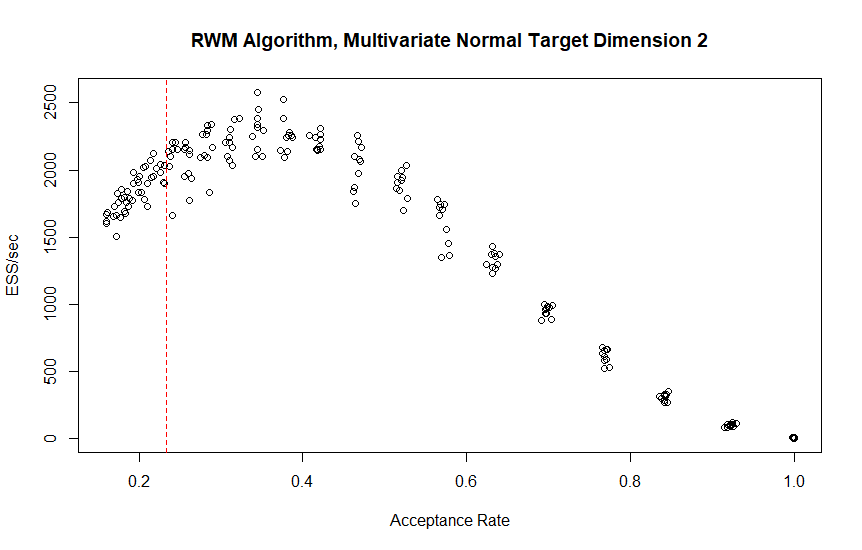
\includegraphics[scale = 0.4]{RWM_Optimal2.png}
\end{figure}

\end{frame}

% ==== 

\begin{frame}{Optimal Acceptance Rate: RWM}
\begin{figure}
\centering
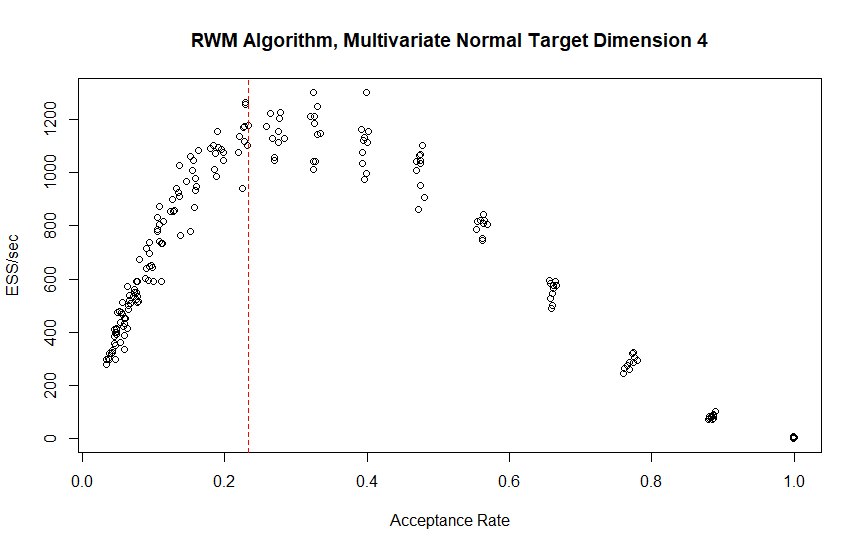
\includegraphics[scale = 0.4]{RWM_Optimal4.png}
\end{figure}
\end{frame}

% ==== 

\begin{frame}{Optimal Acceptance Rate: RWM}
\begin{figure}
\centering
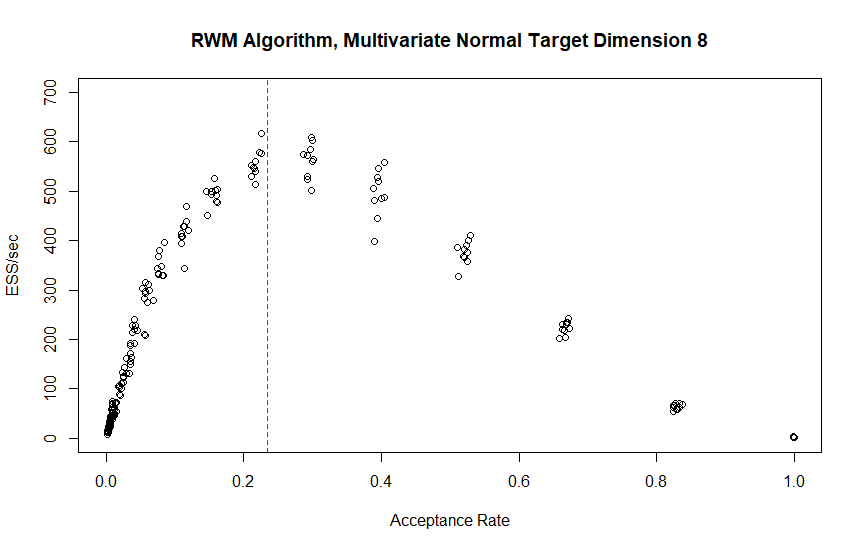
\includegraphics[scale = 0.4]{RWM_Optimal8.png}
\end{figure}
\end{frame}

% ==== 

\begin{frame}{Optimal Acceptance Rate: RWM}
\begin{figure}
\centering
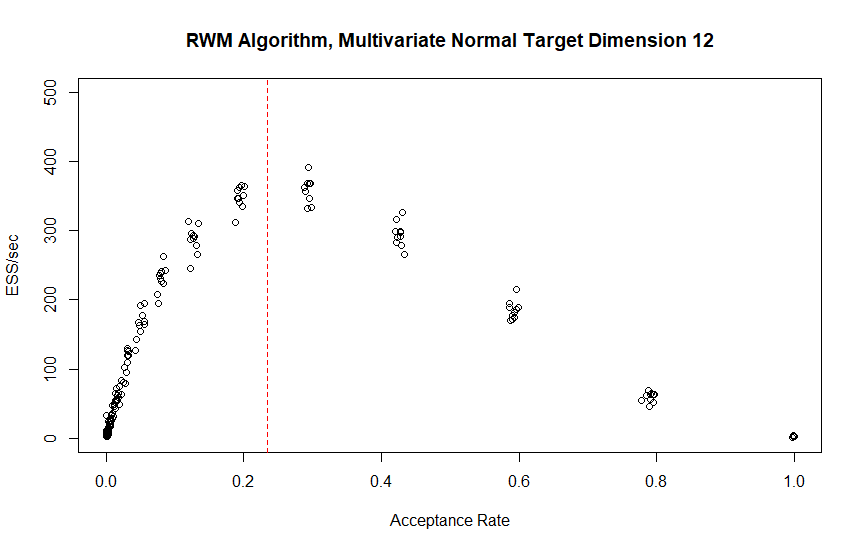
\includegraphics[scale = 0.3]{RWM_Optimal12.png}
\end{figure}
\end{frame}

% ====

\begin{frame}{Optimal Acceptance Rate: HMC}

\begin{figure}
\centering
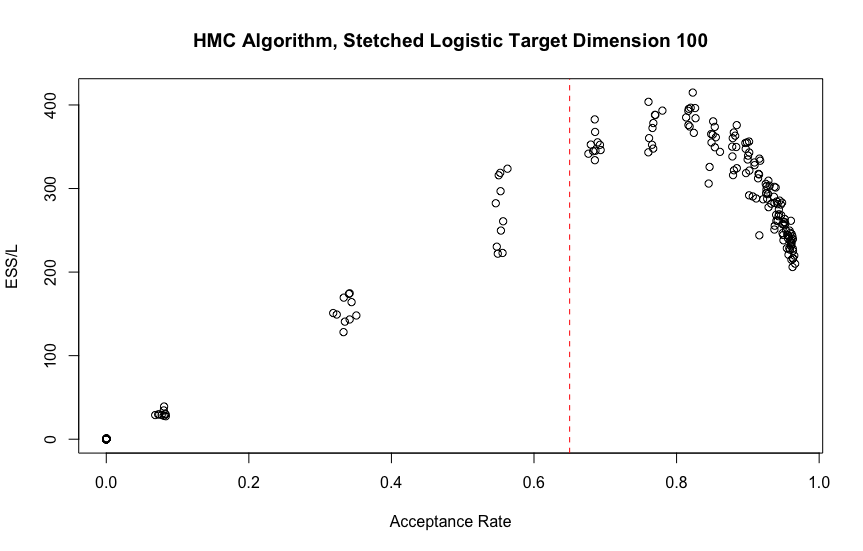
\includegraphics[scale = 0.3]{HMC_Optimal100.png}
\end{figure}

\end{frame}

% ==== 

\begin{frame}{Optimal Acceptance Rate: HMC}
\begin{figure}
\centering
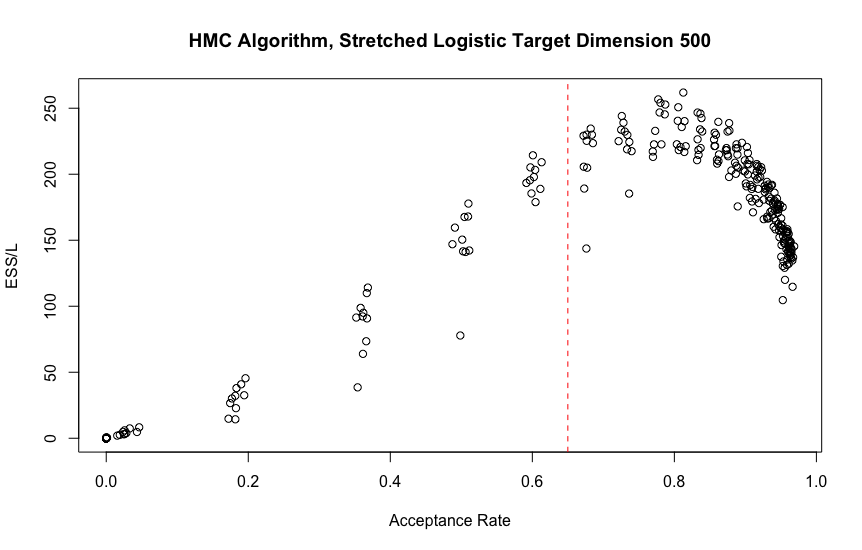
\includegraphics[scale = 0.3]{HMC_Optimal500.png}
\end{figure}
\end{frame}

% ==== 

\begin{frame}{Optimal Acceptance Rate: HMC}
\begin{figure}
\centering
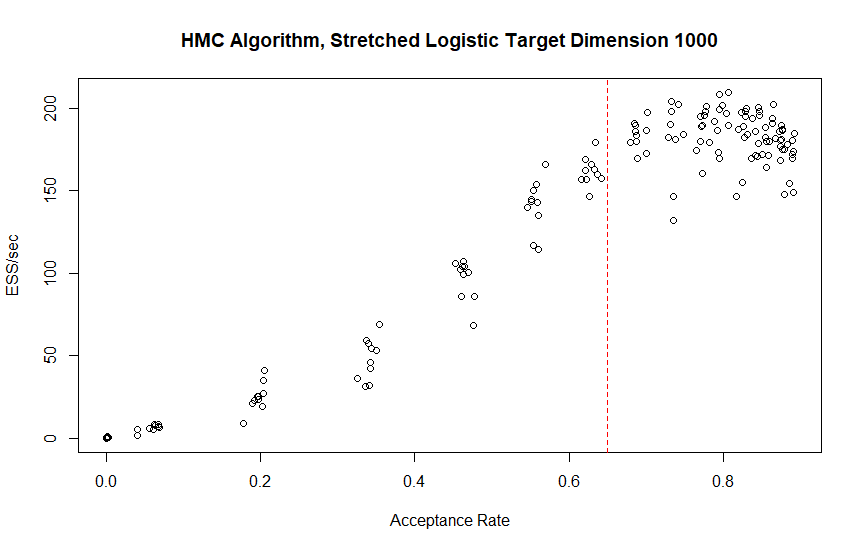
\includegraphics[scale = 0.3]{HMC_Optimal1000.png}
\end{figure}
\end{frame}

% ===============================================

\section{Conclusion}

% ===============================================


\begin{frame}{Further Topics}

\begin{itemize}

\item Reversibility 

\item Störmer-Verlet Approximation 

\item Partial Momentum Refreshment

\item Relativistic Monte Carlo

\end{itemize}

\begin{center}
Thank you for listening.
\vskip 0.5cm
Any Questions?

\end{center}


\end{frame}


\end{document}


\begin{frame}{References}

\begin{enumerate}
\item

\item

\item
\end{enumerate}


\end{frame}


\end{document}
